\begin{frame}
    \frametitle{Формулировка проблемы}
    \textbf{Актуальность.} В настоящее время формирование маршрутов в городской
    среде осуществляется на основе положений, заложенных в городской план
    развития. Обычно, эта информация достаточно устаревшая и не учитывает
    предпочтения жителей. На основе данных о предпочтениях жителей требуется
    разработать эффективный метод кластеризации предпочтений жителей города
    по перемещению.
\end{frame}

\begin{frame} % Слайд 3
    \frametitle{Цели и задачи}
    \textbf{Цель работы} -- разработка метода кластеризации предпочтений
    жителей для минимизации дискомфорта перемещения в городе.\\
    \textbf{Задачи:}
    \begin{itemize}
        \item выбор алгоритма кластеризации;
        \item разработка метода учета географических особенностей местности;
        \item разработка критериев для оценки качества кластеризации;
        \item генерация исходных данных;
        \item визуализация полученных результатов.
    \end{itemize}
\end{frame}

\begin{frame}
    \frametitle{Перемещения}
    \begin{figure}
        \center
        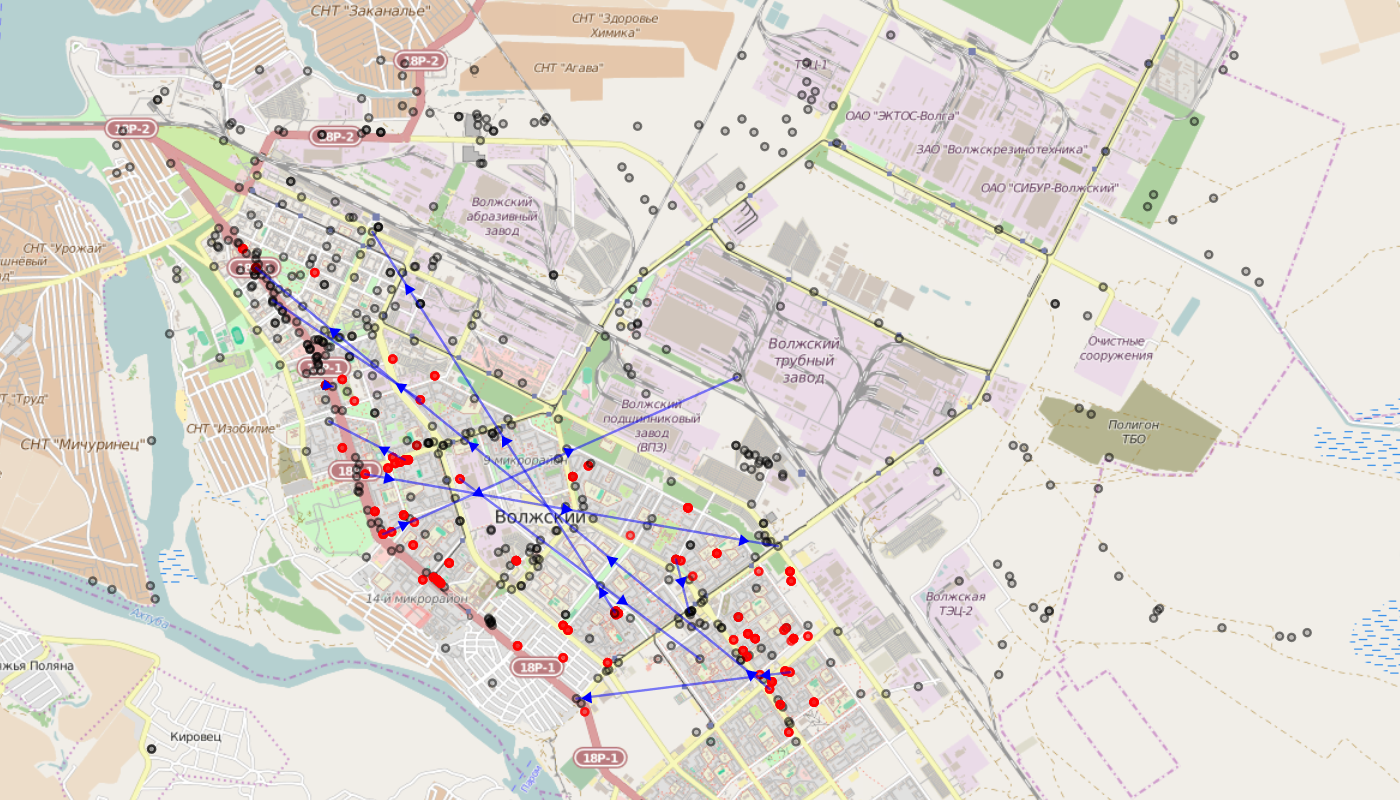
\includegraphics[width=\textwidth]{image01}
    \end{figure}
\end{frame}

\begin{frame}
    \frametitle{Перемещения}
    \begin{figure}
        \center
        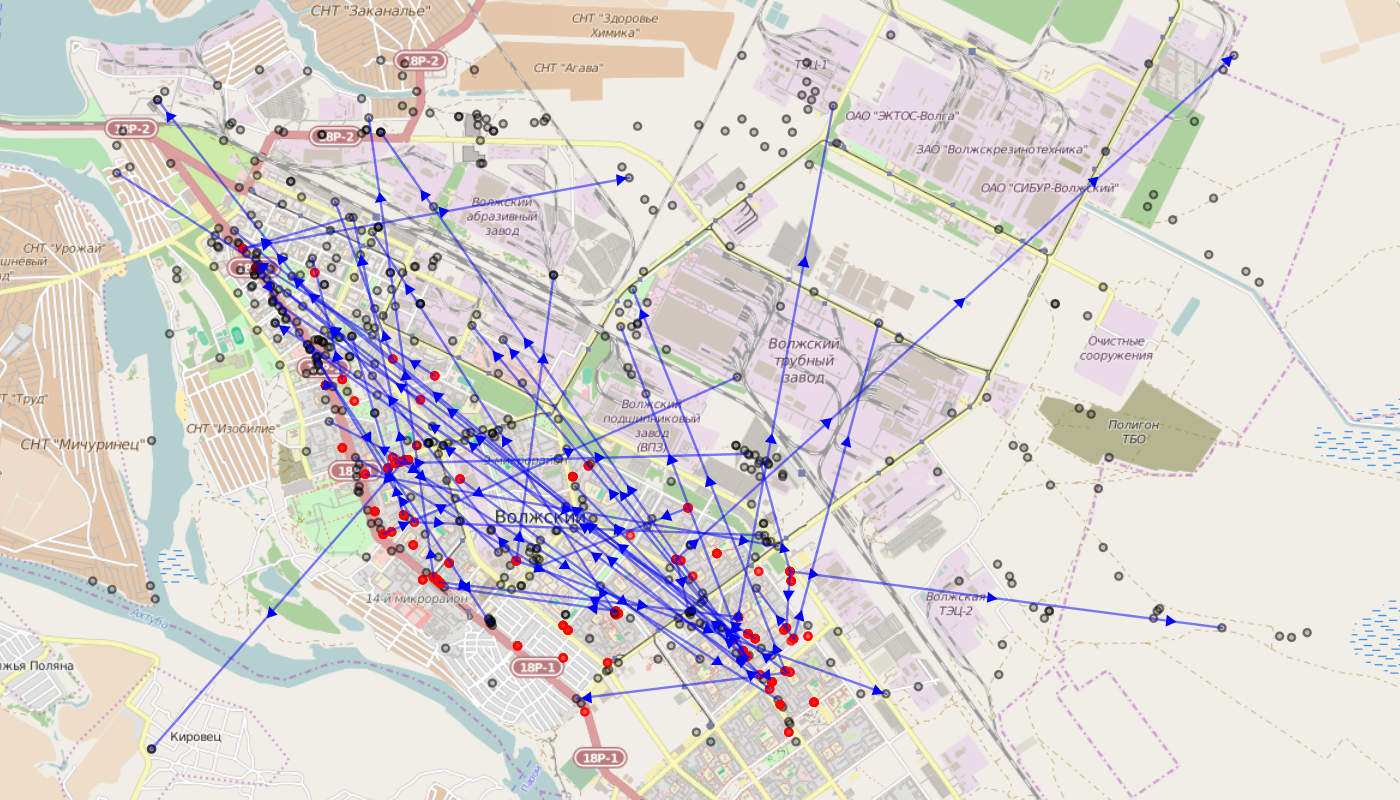
\includegraphics[width=\textwidth]{image02}
    \end{figure}
\end{frame}

\begin{frame}
    \frametitle{Перемещения}
    \begin{figure}
        \center
        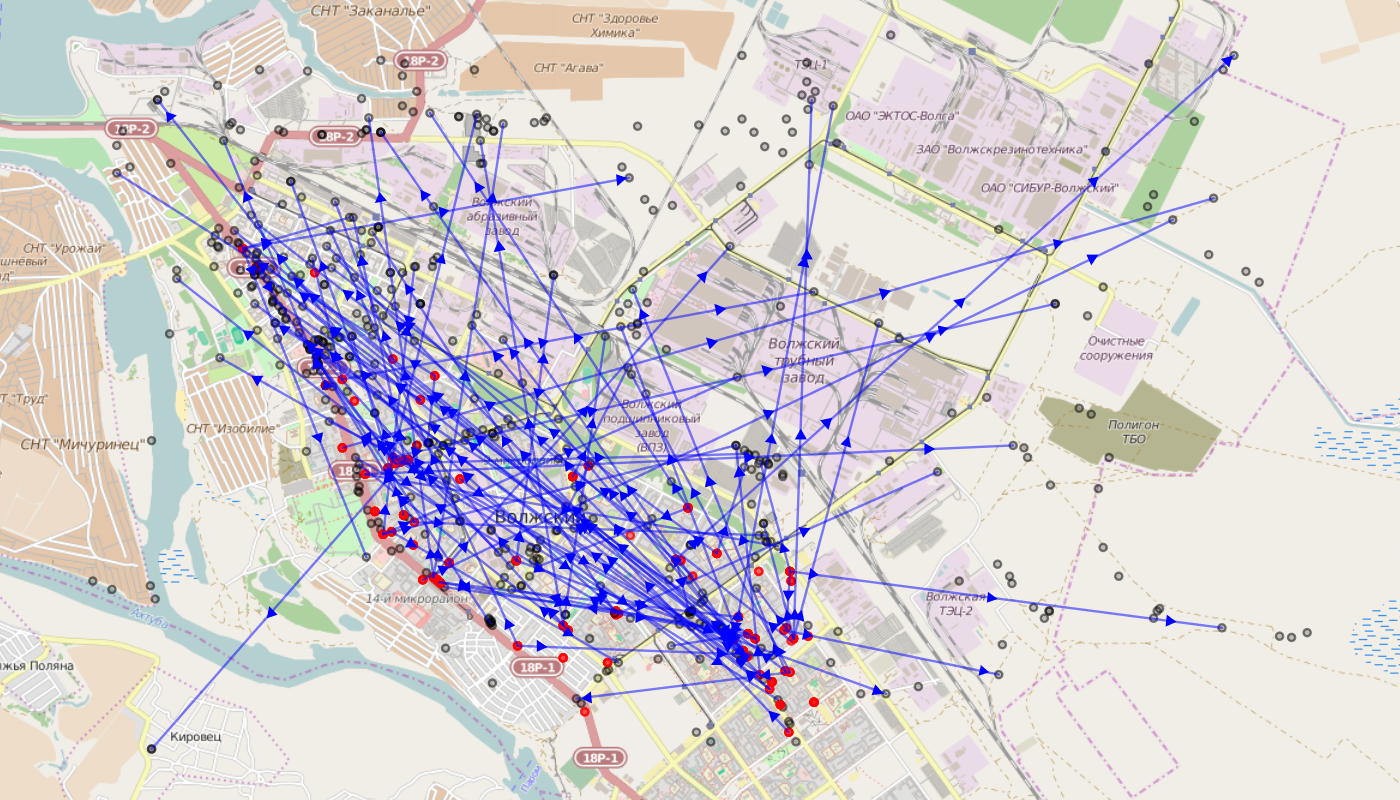
\includegraphics[width=\textwidth]{image03}
    \end{figure}
\end{frame}

\begin{frame}
    \frametitle{Перемещения}
    \begin{figure}
        \center
        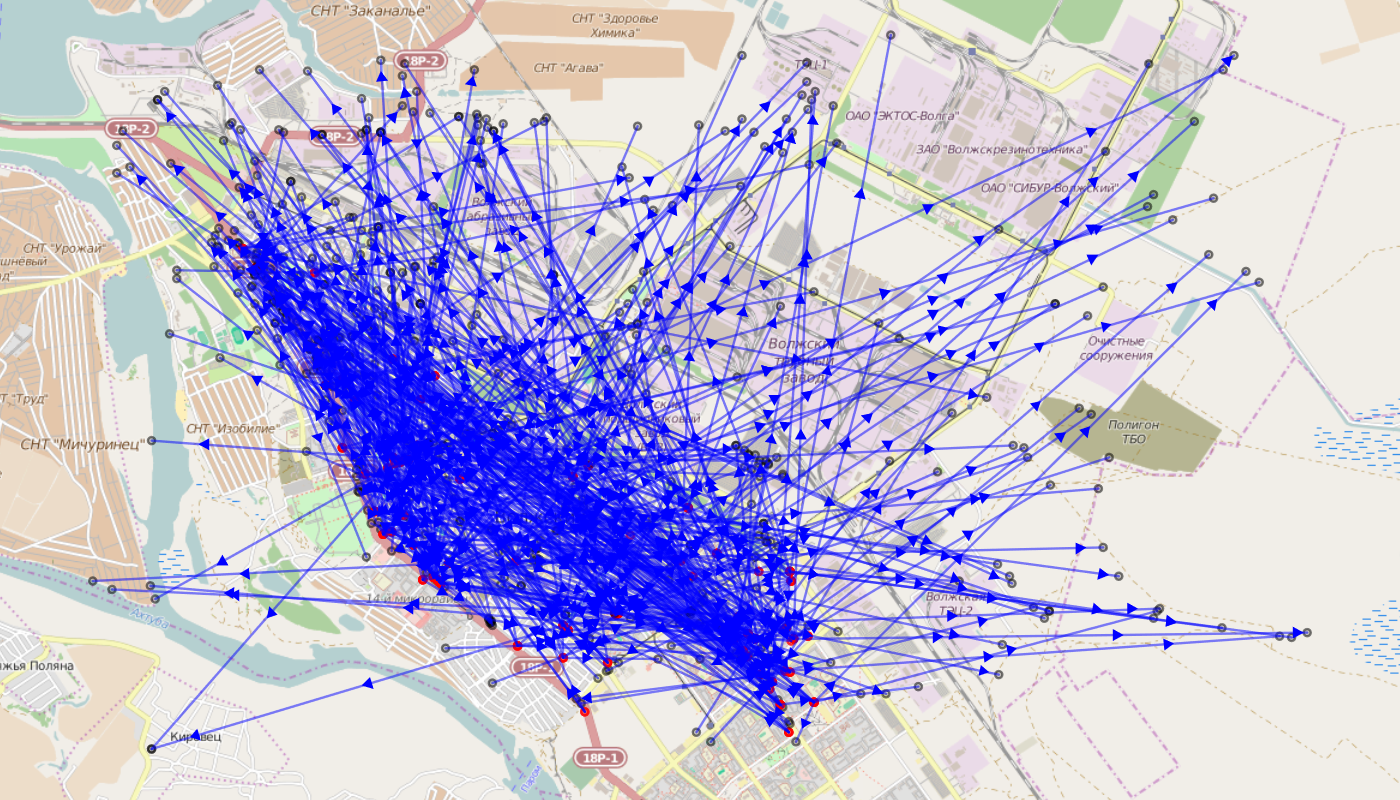
\includegraphics[width=\textwidth]{image04}
    \end{figure}
\end{frame}

\begin{frame}
    \frametitle{Исходная выборка}
    \begin{figure}
        \center
        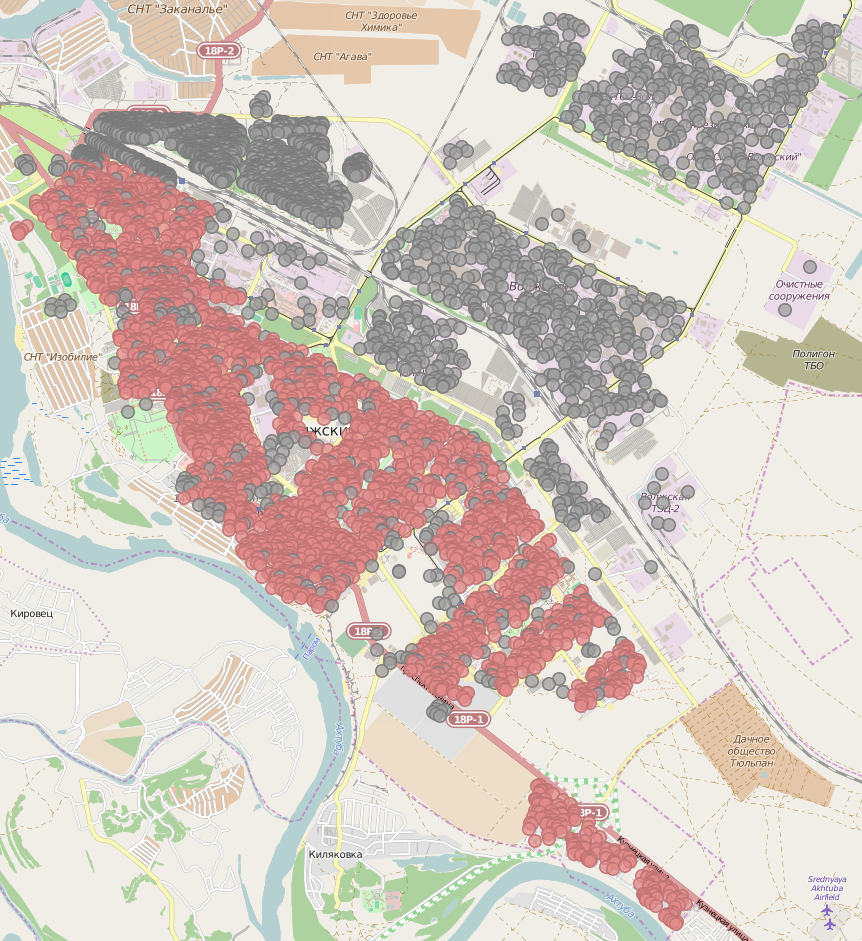
\includegraphics[width=.7\textwidth]{map}
    \end{figure}
\end{frame}

\begin{frame}
    \frametitle{Используемый алгоритм}
    Псевдокод алгоритма K-Means:\\
    \vspace{1em}
    \footnotesize
    \textbf{ВВОД} точки, положение\_центроидов, количество\_итераций\\
    итерация = 0, пред.\_положение = []\\
    \textbf{ДЕЛАТЬ ПОКА} итерация < количество\_итераций
    \textbf{ИЛИ} \\ \hspace{.15cm} пред.\_положение != положение\_центроидов:\\
    \hspace{.5cm} рассчет принадлежности точек\\
    \hspace{.5cm} пред.\_положение = положение\_центроидов\\
    \hspace{.5cm} положение\_центроидов = средние координаты точек,\\
    \hspace{4.8cm}принадлежащих кластеру\\
    \hspace{.5cm} итерация += 1\\
    \textbf{ВЫВОД} положение\_центроидов
\end{frame}

\begin{frame}
    \frametitle{Прототип}
    \begin{figure}
        \center
        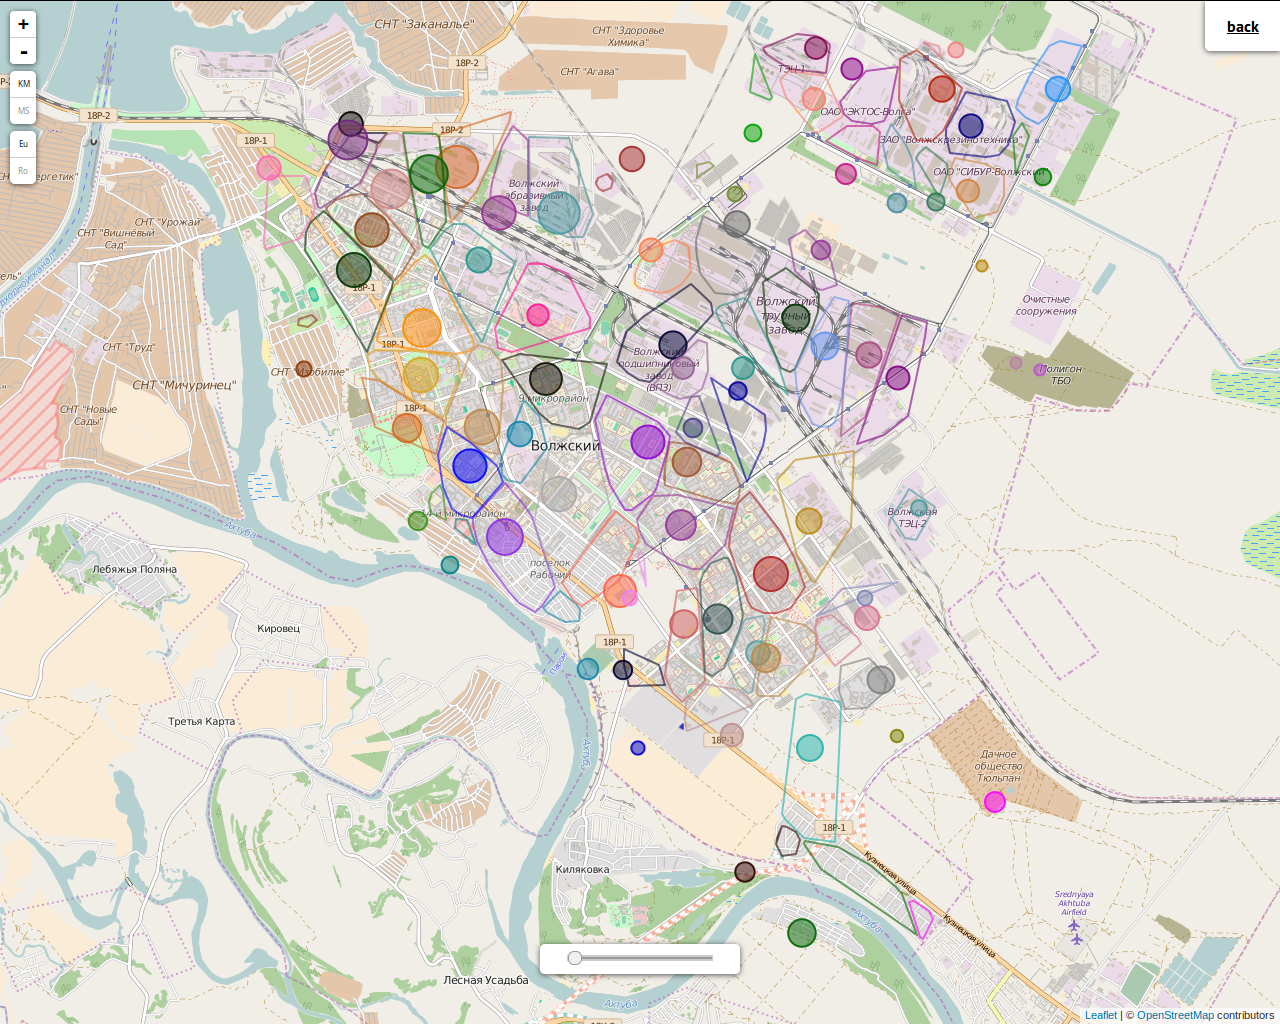
\includegraphics[width=.9\textwidth]{km_before}
    \end{figure}
\end{frame}

\begin{frame}
    \frametitle{Прототип}
    \begin{figure}
        \center
        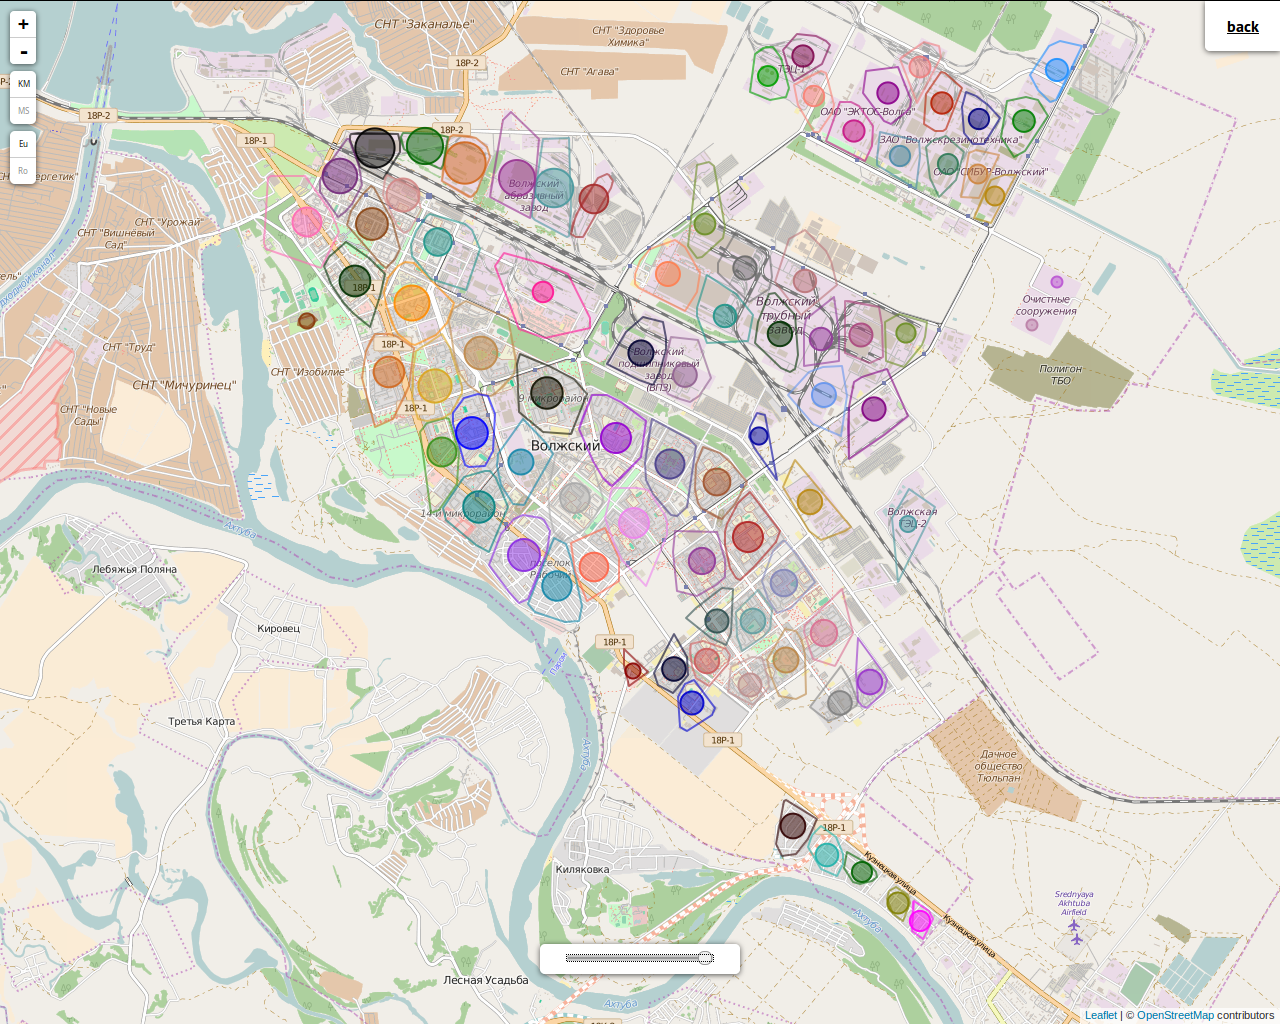
\includegraphics[width=.9\textwidth]{km_after}
    \end{figure}
    \small\emph{Ссылка на приложение:} \url{http://vstu-cad-stuff.github.io/clustering/}
\end{frame}

\begin{frame}
    \frametitle{Метрика}
    Пример использования движка OSRM:
    \begin{figure}
        \center
        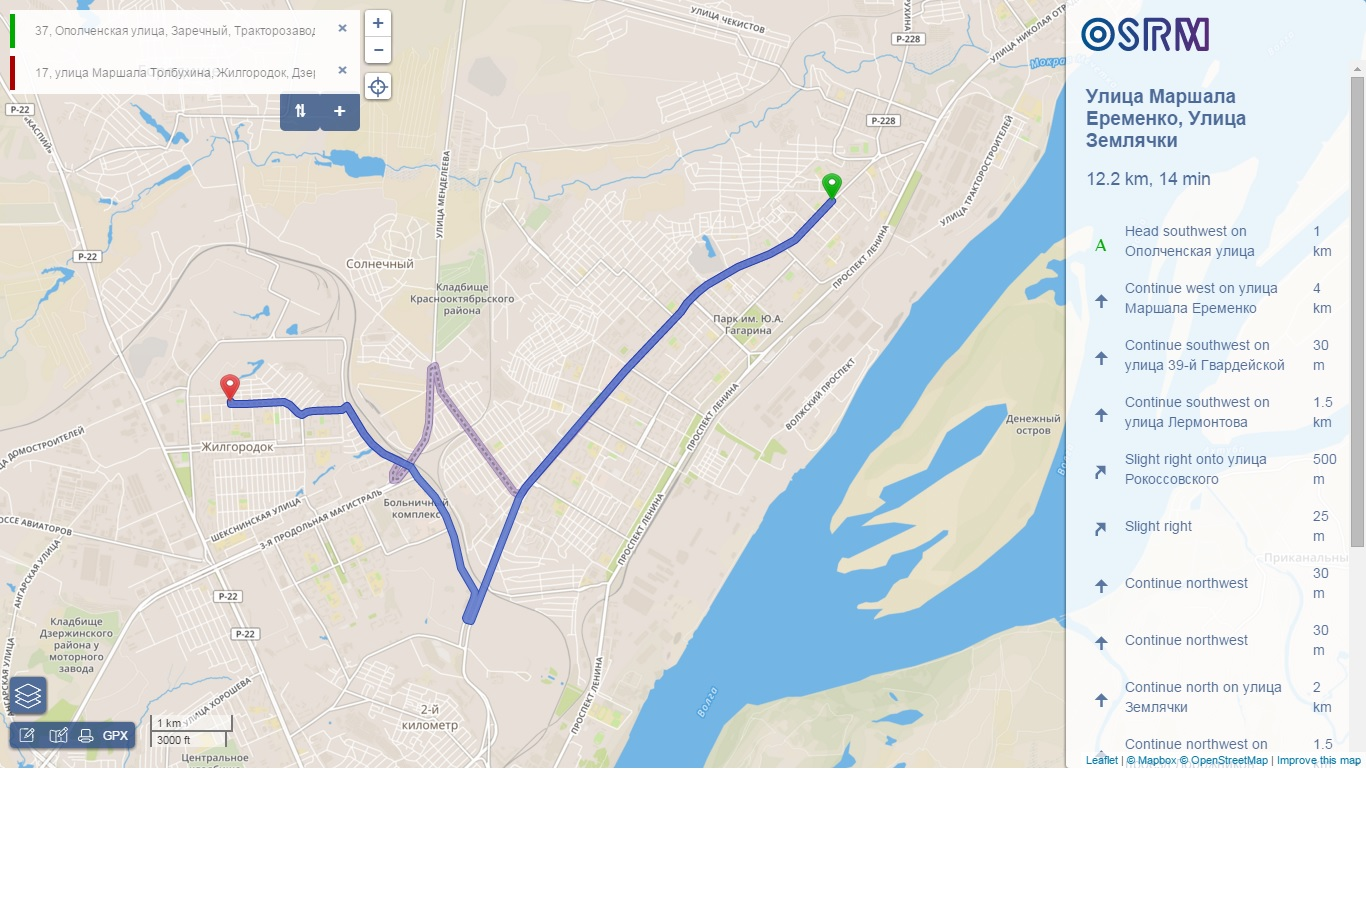
\includegraphics[width=\textwidth]{osrm}
    \end{figure}
\end{frame}

\begin{frame}
    \frametitle{Построение маршрутов}
    \begin{figure}
        \center
        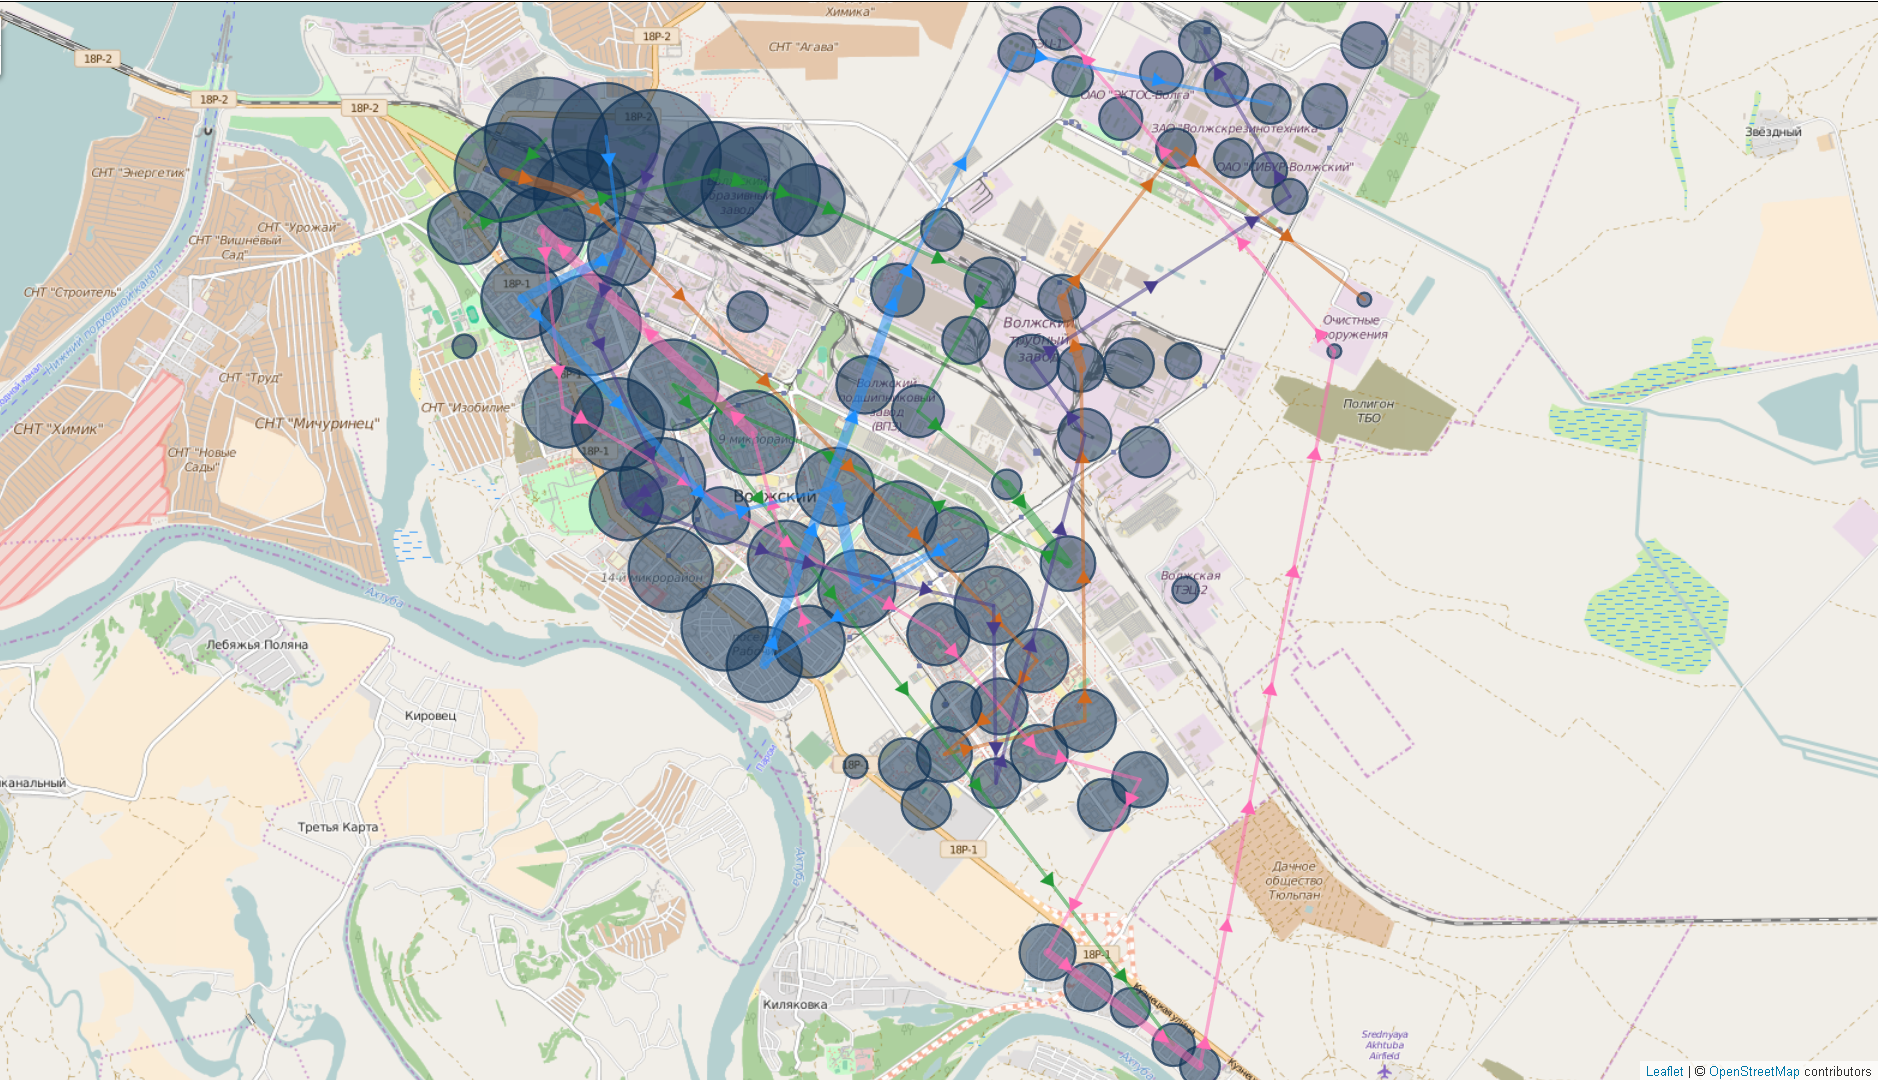
\includegraphics[width=\textwidth]{clusters_02}
    \end{figure}
    \small\emph{Ссылка на приложение:} \url{http://vstu-cad-stuff.github.io/routing/}
\end{frame}
